\subsection{Màn hình Menu của Client}
\subsubsection{Mô tả}
Dưới đây là nội dung hiển thị của màn hình Menu tương ứng với vai trò \textbf{Admin} (\textbf{Client}). Ở màn hình menu của Client, ứng dụng hỗ trợ 2 chức năng cơ bản: Thêm một người dùng mới vào danh sách kết nối (nút \textbf{Add new user}), kết nối trực tiếp đến một người dùng nào đó (\textbf{Connect to user}). (Hình \ref{fig:ClientMenuWindow})
\begin{figure}[H]
	\centering{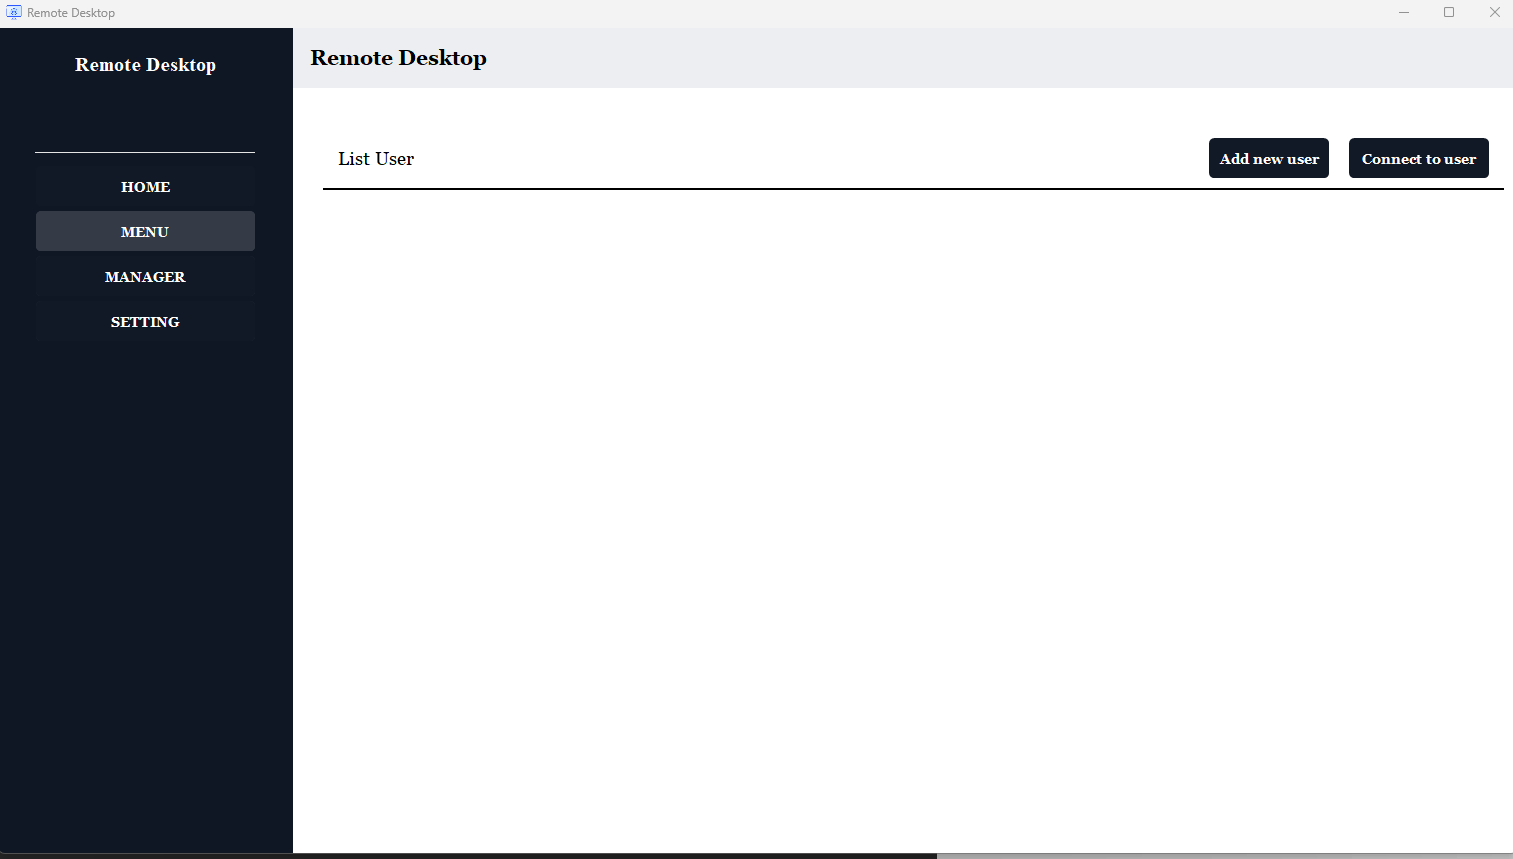
\includegraphics[scale=0.4]{ClientMenuWindow}}
	\caption{Màn hình chính của ứng dụng}
	\label{fig:ClientMenuWindow}
\end{figure}
\subsubsection{Thêm một người dùng mới vào danh sách các kết nối (nút Add new user)}
Khi ta sử dụng chức năng \textbf{Add new user}, hộp thoại \textbf{Add new user} xuất hiện với 2 trường thông tin cần nhập đó là ``User Id'' và ``User IP Address''. Trường ``User Id'' yêu cầu ta nhập tên nhận dạng, trường này có kiểu dữ liệu là \verb|std::string|, mục đích của việc điền thông tin này là để lưu lại tên cụ thể trên danh sách các User nằm ở bên dưới để cho ta dễ nhận biết tên User ta muốn kết nối. Ở trường ``User IP Address'', ta nhập địa chỉ IP của máy cần được kết nối (Hình \ref{fig:AddNewUserBox}). 

\begin{figure}[H]
	\centering{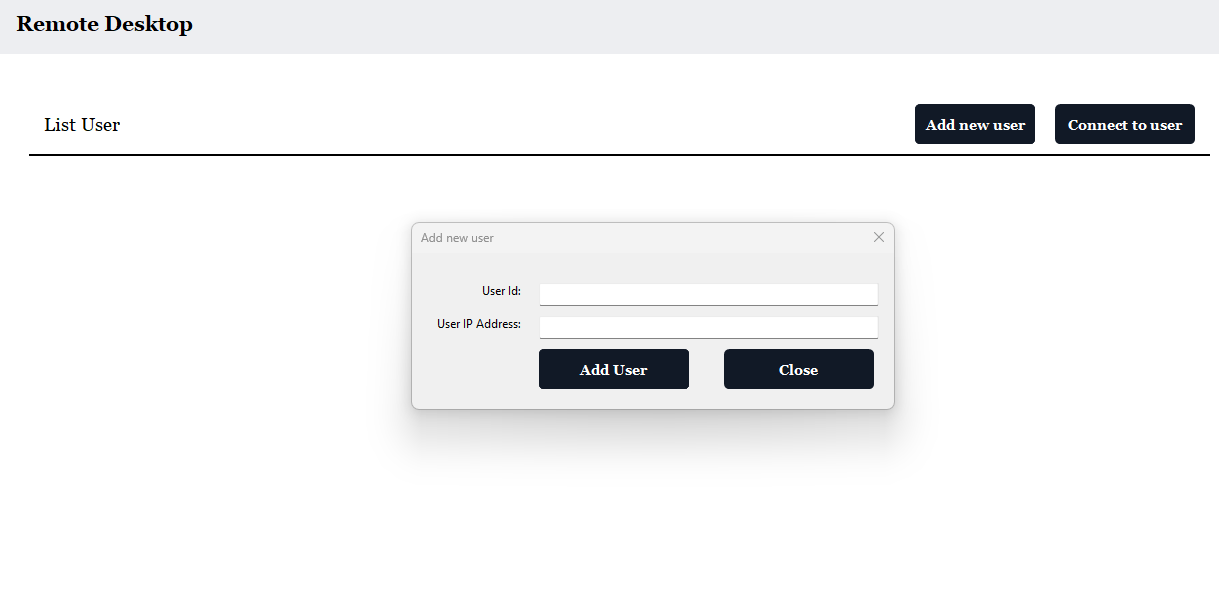
\includegraphics[scale=0.5]{AddNewUserBox}}
	\caption{Hộp thoại Add new user}
	\label{fig:AddNewUserBox}
\end{figure}

Sau khi nhập xong, ta ấn nút ``Add user'' ở góc trái để thêm một người dùng mới vào danh sách kết nối bên dưới. Sau khi thêm một vài người dùng vào danh sách kết nối thì màn hình Menu sẽ có hiển thị như sau. (Hình \ref{fig:UserList})

\begin{figure}[H]
	\centering{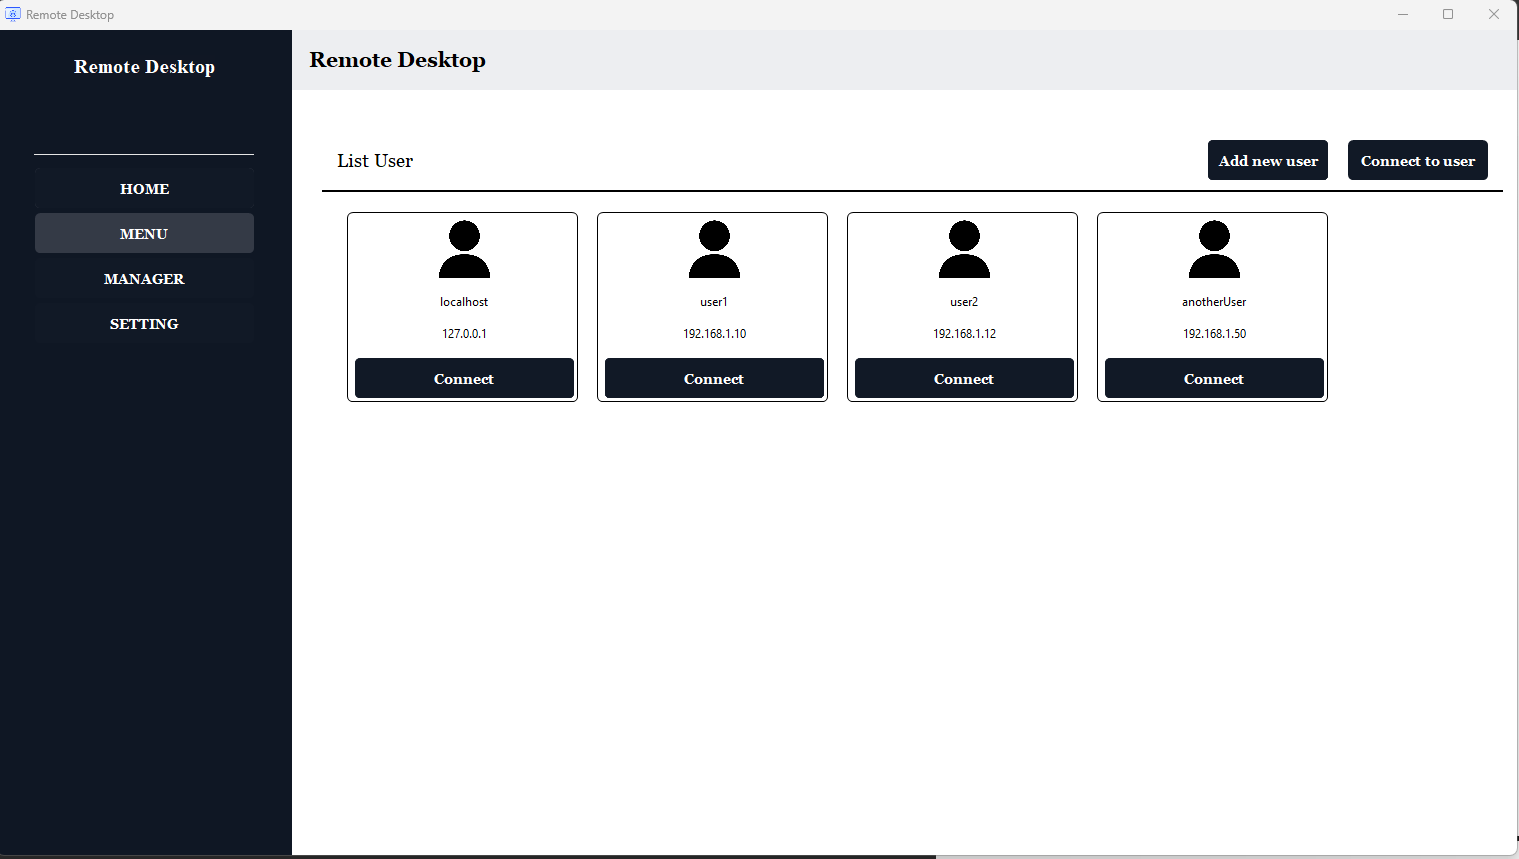
\includegraphics[scale=0.4]{UserList}}
	\caption{Danh sách các user sau khi nhập}
	\label{fig:UserList}
\end{figure}

\subsubsection{Kết nối đến Server (nút Connect/Connect to user)}
Để kết nối đến server, ta có 2 cách để thực hiện: Sử dụng nút ``Connect to user'' ngay bên cạnh ``Add new User'' hoặc nút ``Connect'' ngay bên dưới user tương ứng trong danh sách User trong hình \ref{fig:UserList}.

Nếu ta sử dụng lựa chọn ``Connect to user'', hộp thoại hiện lên với cấu trúc tương tự hộp thoại ``Add new user'', chỉ khác là ở góc trái hiển thị lựa chọn ``Connect to user''. (Hình \ref{fig:ConnectToUserBox})

\begin{figure}[H]
	\centering{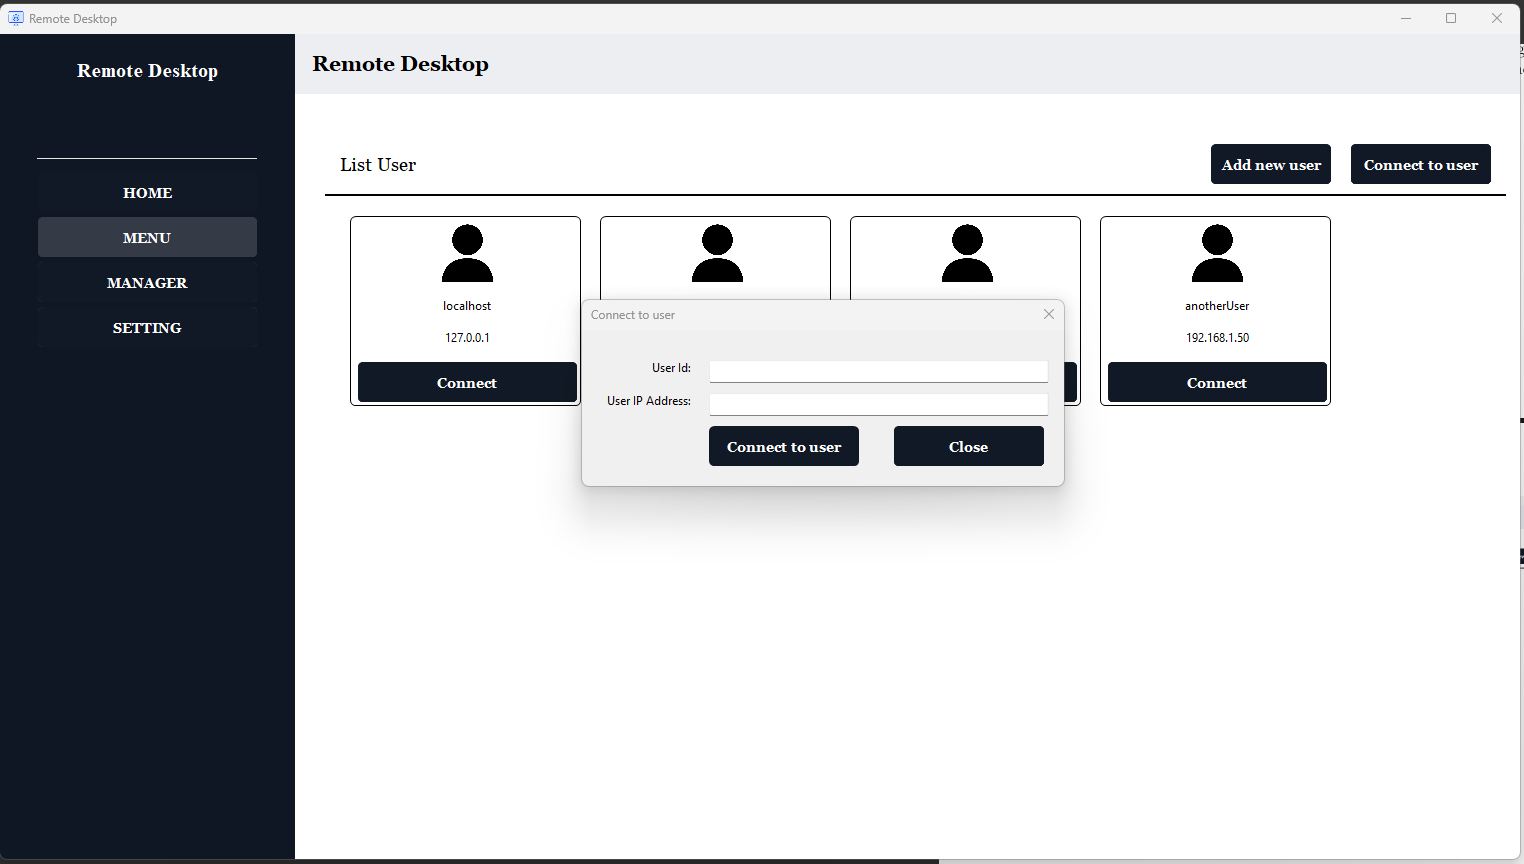
\includegraphics[scale=0.4]{ConnectToUserBox}}
	\caption{Hộp thoại Connect to user}
	\label{fig:ConnectToUserBox}
\end{figure}

Nếu ta sử dụng lựa chọn ``Connect'' bên dưới user cần kết nối trong danh sách User, ta chỉ nhấn vào nút ``Connect'' tương ứng.

Sau khi nhập địa chỉ IP thích hợp và nhấn kết nối, sẽ có hai cửa sổ hiện ra với tiêu đề tương ứng là ``Client Logger'' và ``Client Window''. Nếu kết nối thất bại, 2 cửa sổ này sẽ không có thông tin gì trên đó, cửa sổ Logger sẽ không ghi thông tin gì và cửa sổ ``Client Window'' sẽ không hiển thị màn hình của máy Server (Hình \ref{fig:ClientWindowFailed}). Khi gặp trường hợp trên, ta tắt cửa sổ ``Client Window'' để đóng kết nối hiện tại và quay lại cửa sổ Menu sử dụng lệnh ``Connect'' để thiết lập kết nối mới.

\begin{figure}[H]
	\centering{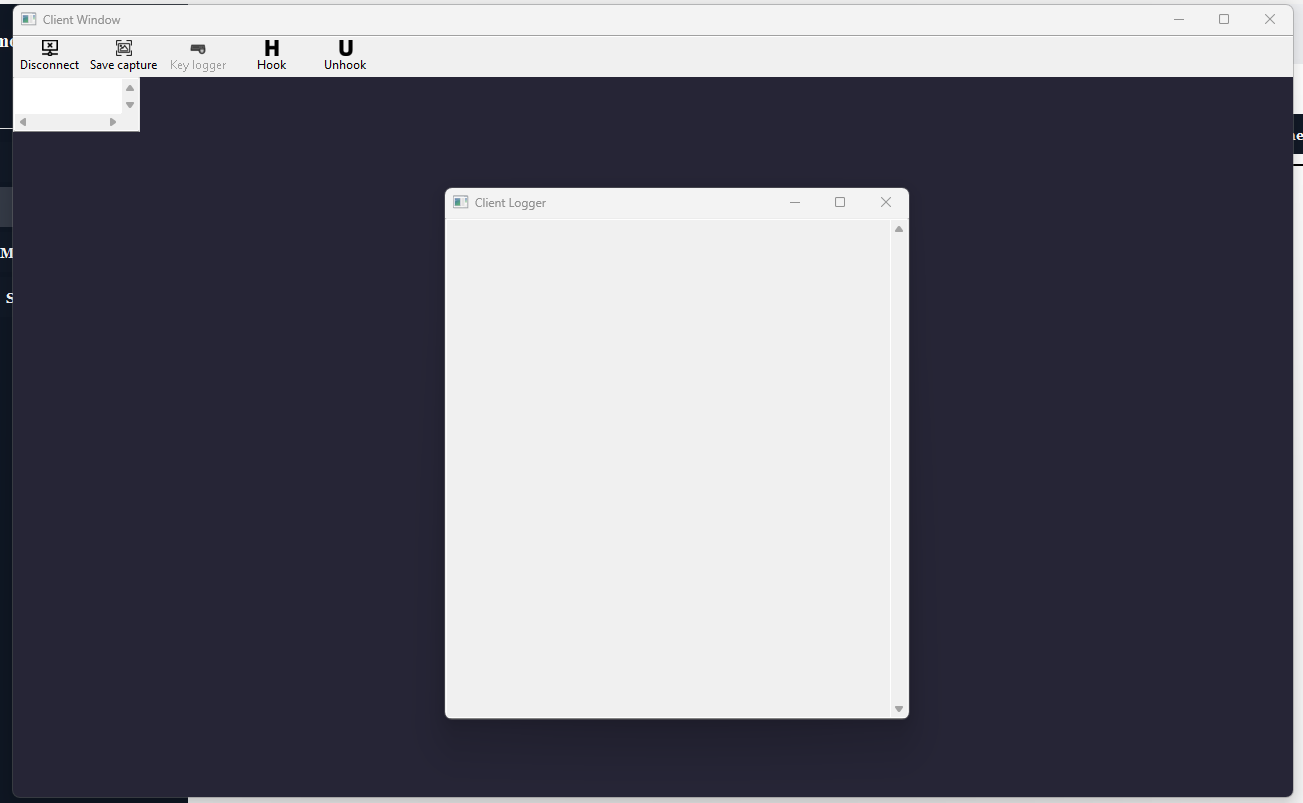
\includegraphics[scale=0.4]{ClientWindowFailed}}
	\caption{Cửa sổ Client Window khi kết nối không thành công}
	\label{fig:ClientWindowFailed}
\end{figure}

Nếu kết nối thành công, cửa sổ ``Client Window'' sẽ hiển thị màn hình của máy được kết nối, trong khi cửa sổ ``Client Logger'' sẽ cung cấp thông tin cơ bản về máy chủ được kết nối (Hình \ref{fig:ClientWindowConnected}). Thông tin này bao gồm địa chỉ IP, địa chỉ MAC và tên cửa sổ của máy chủ. Ở đây, thông tin về máy chủ xuất hiện hai lần vì client thiết lập hai kết nối tới server: một kết nối được sử dụng để nhận hình ảnh và một kết nối khác được dùng để truyền tín hiệu điều khiển.

\begin{figure}[H]
	\centering{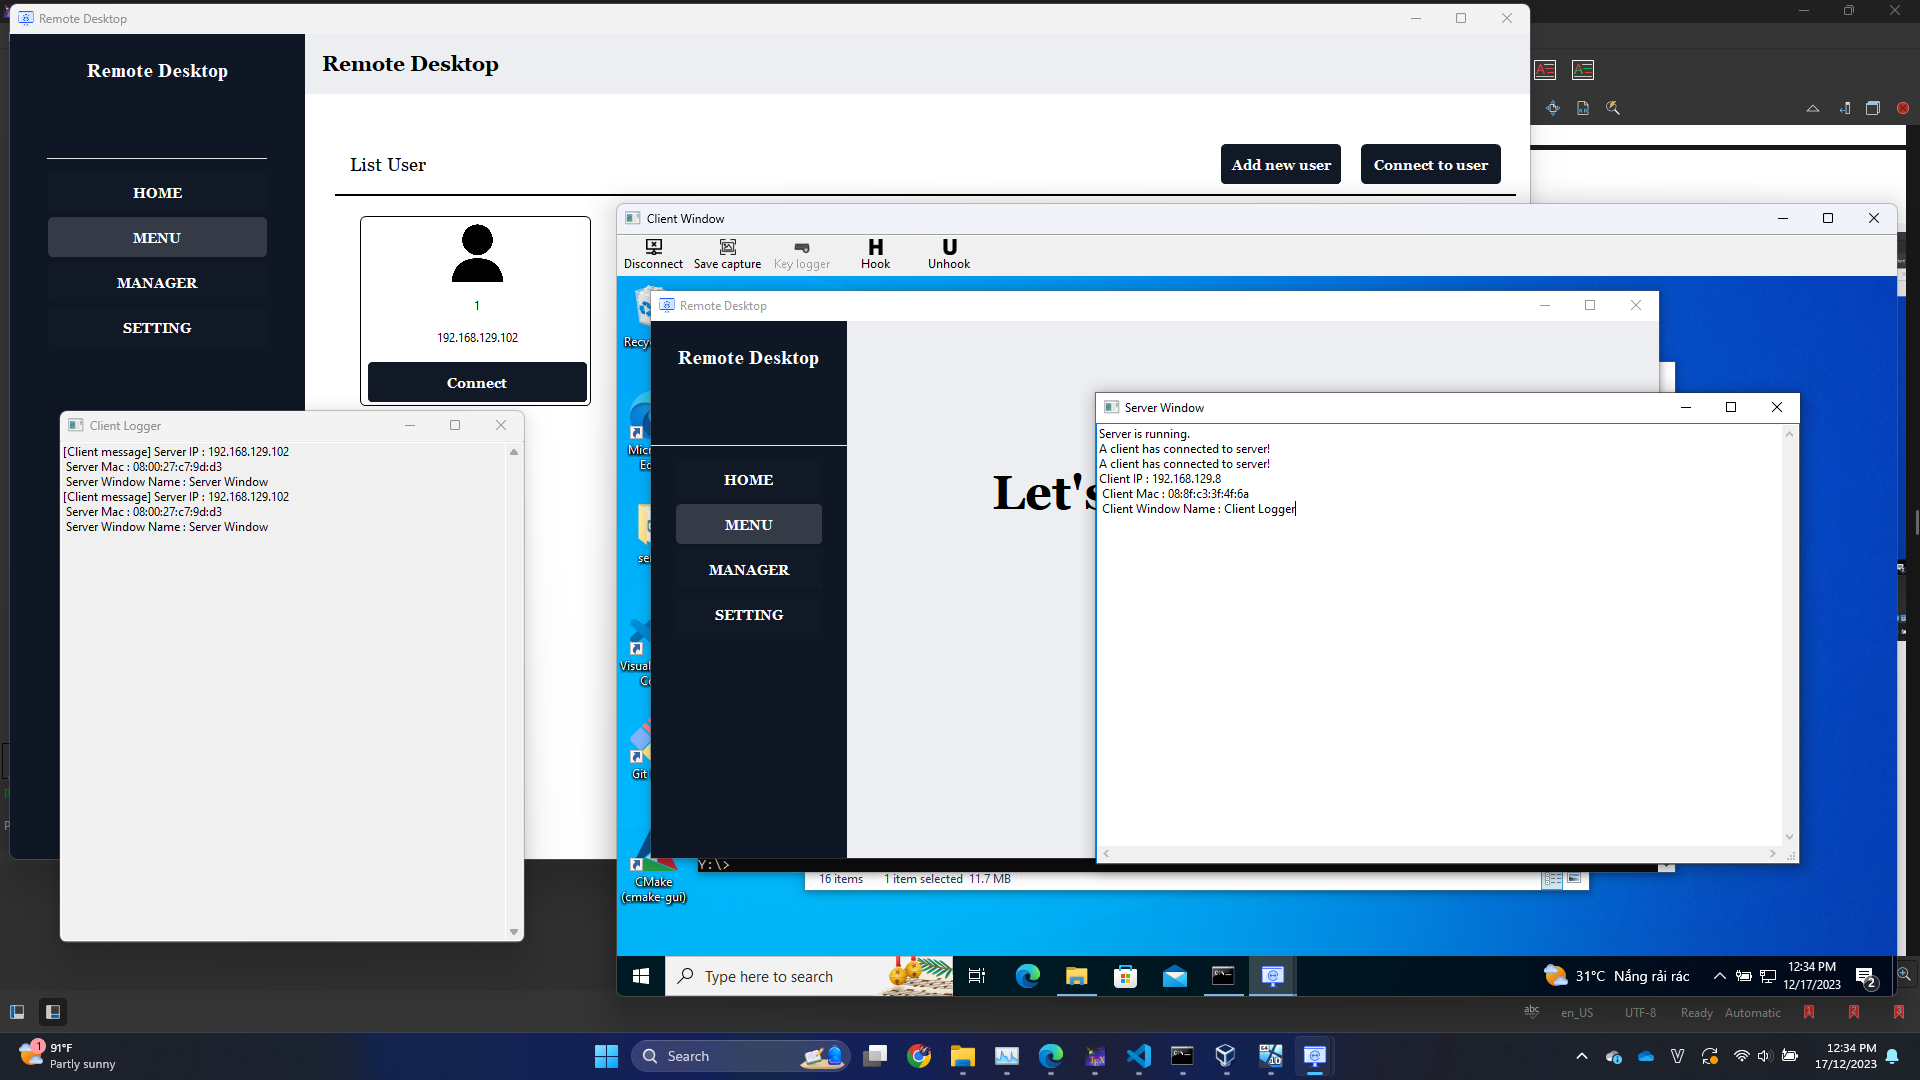
\includegraphics[scale=0.25]{ClientWindowConnected}}
	\caption{Cửa sổ Client Window khi đã thiết lập được kết nối đến một Server}
	\label{fig:ClientWindowConnected}
\end{figure}

Một số lưu ý khi kết nối:
\begin{itemize}
	\item  Kết nối 2 ứng dụng trên 2 máy khác nhau trong cùng mạng: người dùng phía Client cần biết trước IP của máy Server. IP của máy Server có thể lấy ra bằng lệnh \verb|ipconfig| của \textbf{Command Prompt}.
	\item Kết nối 2 ứng dụng trên cùng 1 máy: ngoài cách trên, còn có thể nhập địa chỉ loopback \textbf{127.0.0.1}. Đây là địa chỉ IP đặc biệt được dùng để tham chiếu đến chính máy tính đang sử dụng. Khi gửi dữ liệu đến địa chỉ loopback, dữ liệu sẽ được gửi và xử lý trên cùng một máy tính mà không cần thông qua mạng vật lý.
	\item Mỗi Client \textbf{chỉ điều khiển} được 1 Server ở tại một thời điểm. Điều này có nghĩa là, khi muốn điều khiển máy khác, Client phải ngắt kết nối với Server hiện tại để có thể thiết lập kết nối mới với máy khác.
\end{itemize}

\subsubsection{Ngắt kết nối với Server (nút Disconnect)}
Để sử dụng chức năng này, trước hết phía người dùng phía Client cần nhấn nút ``Disconnect'' trên thanh Toolbar của Client Window. Một hộp thoại lúc này sẽ hiện ra, yêu cầu ta xác nhận về việc có ngắt kết nối đến Server và đồng thời tắt Client Window hay không (Hình \ref{fig:ClientDisconnectDialog}). Nếu xác nhận ngắt kết nối, cửa sổ Client Window và Client Logger sẽ được đóng đồng thời kết nối từ Client đến Server sẽ không còn.

\begin{figure}[H]
	\centering{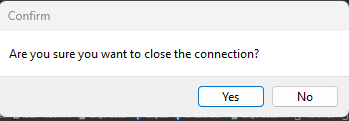
\includegraphics[scale=1]{ClientDisconnectDialog}}
	\caption{Hộp thoại xác nhận ngắt kết nối ở phía Client}
	\label{fig:ClientDisconnectDialog}
\end{figure}

\subsubsection{Chụp màn hình Server (nút Save Capture)}\label{subsubsec:saveCapture}
Để sử dụng chức năng này, trước hết người dùng phía Client cần nhấn nút ``Save Capture''. Sau khi ấn xong, hình ảnh sẽ được lưu vào thư mục ``CURRENT\_FOLDER\slash Screenshots" với ``CURRENT\_FOLDER'' là thư mục đang đứng để gọi ứng dụng Remote Desktop Control (Hình \ref{fig:ScreenshotsDirectory}). Hình ảnh được lưu với cú pháp \newline \noindent \verb|dd-mm-yyyy hh-mm-ss screenshot.png|. 

\begin{figure}[H]
	\centering{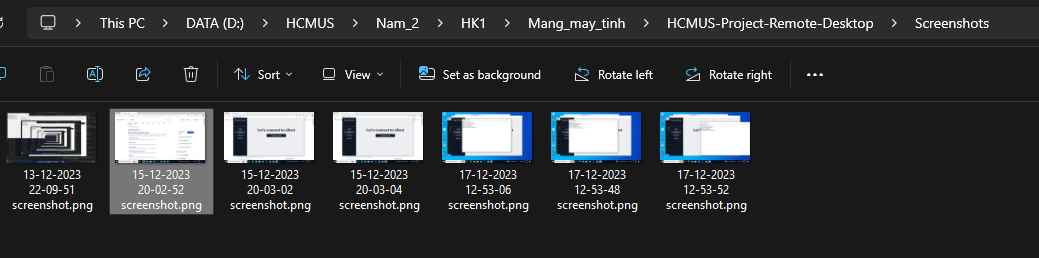
\includegraphics[scale=0.6]{ScreenshotsDirectory}}
	\caption{Các ảnh chụp màn hình đã được lưu trong thư mục Screenshots}
	\label{fig:ScreenshotsDirectory}
\end{figure}

\subsubsection{Gửi tín hiệu điều khiển cho Server}
Sau khi thiết lập kết nối thành công, Client lúc này sẽ nhận được hình ảnh màn hình hiện tại của Server và bắt đầu điều khiển từ xa. Máy Client có thể điều khiển chuột và bàn phím của máy Server trong suốt quá trình kết nối. Tuy nhiên, sẽ có những phím đặc biệt mà máy Client không gửi được cho Server, vấn đề này sẽ được giải quyết trong \ref{sec:HookUnhookSection}.

\subsubsection{Gửi các tín hiệu phím đặc biệt đến cho Server (nút Hook/Unhook)}\label{sec:HookUnhookSection}
Trong quá trình gửi các tín hiệu bàn phím, có những phím đặc biệt mà Client không thể gửi được cho Server một cách trọn vẹn vì mọi tín hiệu bàn phím sẽ được hệ điều hành nhận và xử lí đầu tiên, do đó đối với những phím có những chức năng đặc biệt như \textbf{Windows} hoặc tổ hợp phím \textbf{Alt + Tab} thì cần có những công cụ riêng để xử lí. Do đó, nhóm đã tạo chức năng \textbf{Hook/Unhook} ở máy Client với vai trò là bắt những tín hiệu phím đặc biệt như trên và gửi cho phía Server thực hiện hành động nhấn phím đó.

\begin{figure}[H]
	\centering{\includegraphics[scale=1]{HookUnHookButtons}}
	\caption{Phím Hook và Unhook trên thanh Toolbar của Client Window}
	\label{fig:HookUnHookButtons}
\end{figure}

Để sử dụng chức năng \textbf{Hook}, ta nhấn vào phím ``Hook'' trên thanh Toolbar của cửa sổ ``Client Window''. Sau khi nhấn phím ``Hook'' xong, các phím đặc biệt như ``Windows'', ``Alt'', ``Esc'' sẽ được nhận và gửi cho Server khi ta nhấn các phím các phím đó xuống mà không bị gián đoạn vì hệ điều hành của máy Client xử lí phím đó trước.

Để ngừng sử dụng chức năng \text{Hook}, ta nhấn phím ``Unhook'', dừng việc bắt các sự kiện phím đặc biệt để gửi cho Server, lúc này phía Server sẽ không nhận được những phím đặc biệt đó mà máy của Client vẫn nhận được phím đó bình thường.